\section{Model Families of Satellite Embeddings}

The current \texttt{rs-embed} workspace exposes \modelcount{} canonical models, and the accompanying dossier records their publication metadata, supported sensors, output forms, and runtime summaries. For a review article, however, the reader should not face these as a flat inventory. A more natural structure is to first divide the field into a few broad model families, then summarize the common architecture and data logic of each family, and only after that return to a unified comparison table.

\subsection{Family I: Precomputed embedding products}

This family treats the embedding itself as a distributed geospatial product rather than as a checkpoint that must be run by the user. Examples include GSE, TESSERA, and Copernicus-style feature maps \citep{gse,tessera,copernicus}. Their main strengths are immediate access, large-area consistency, and low inference burden at use time. Their main limitations are temporal rigidity, storage requirements, and dependence on a fixed upstream production workflow.

\begin{figure}[t]
  \centering
  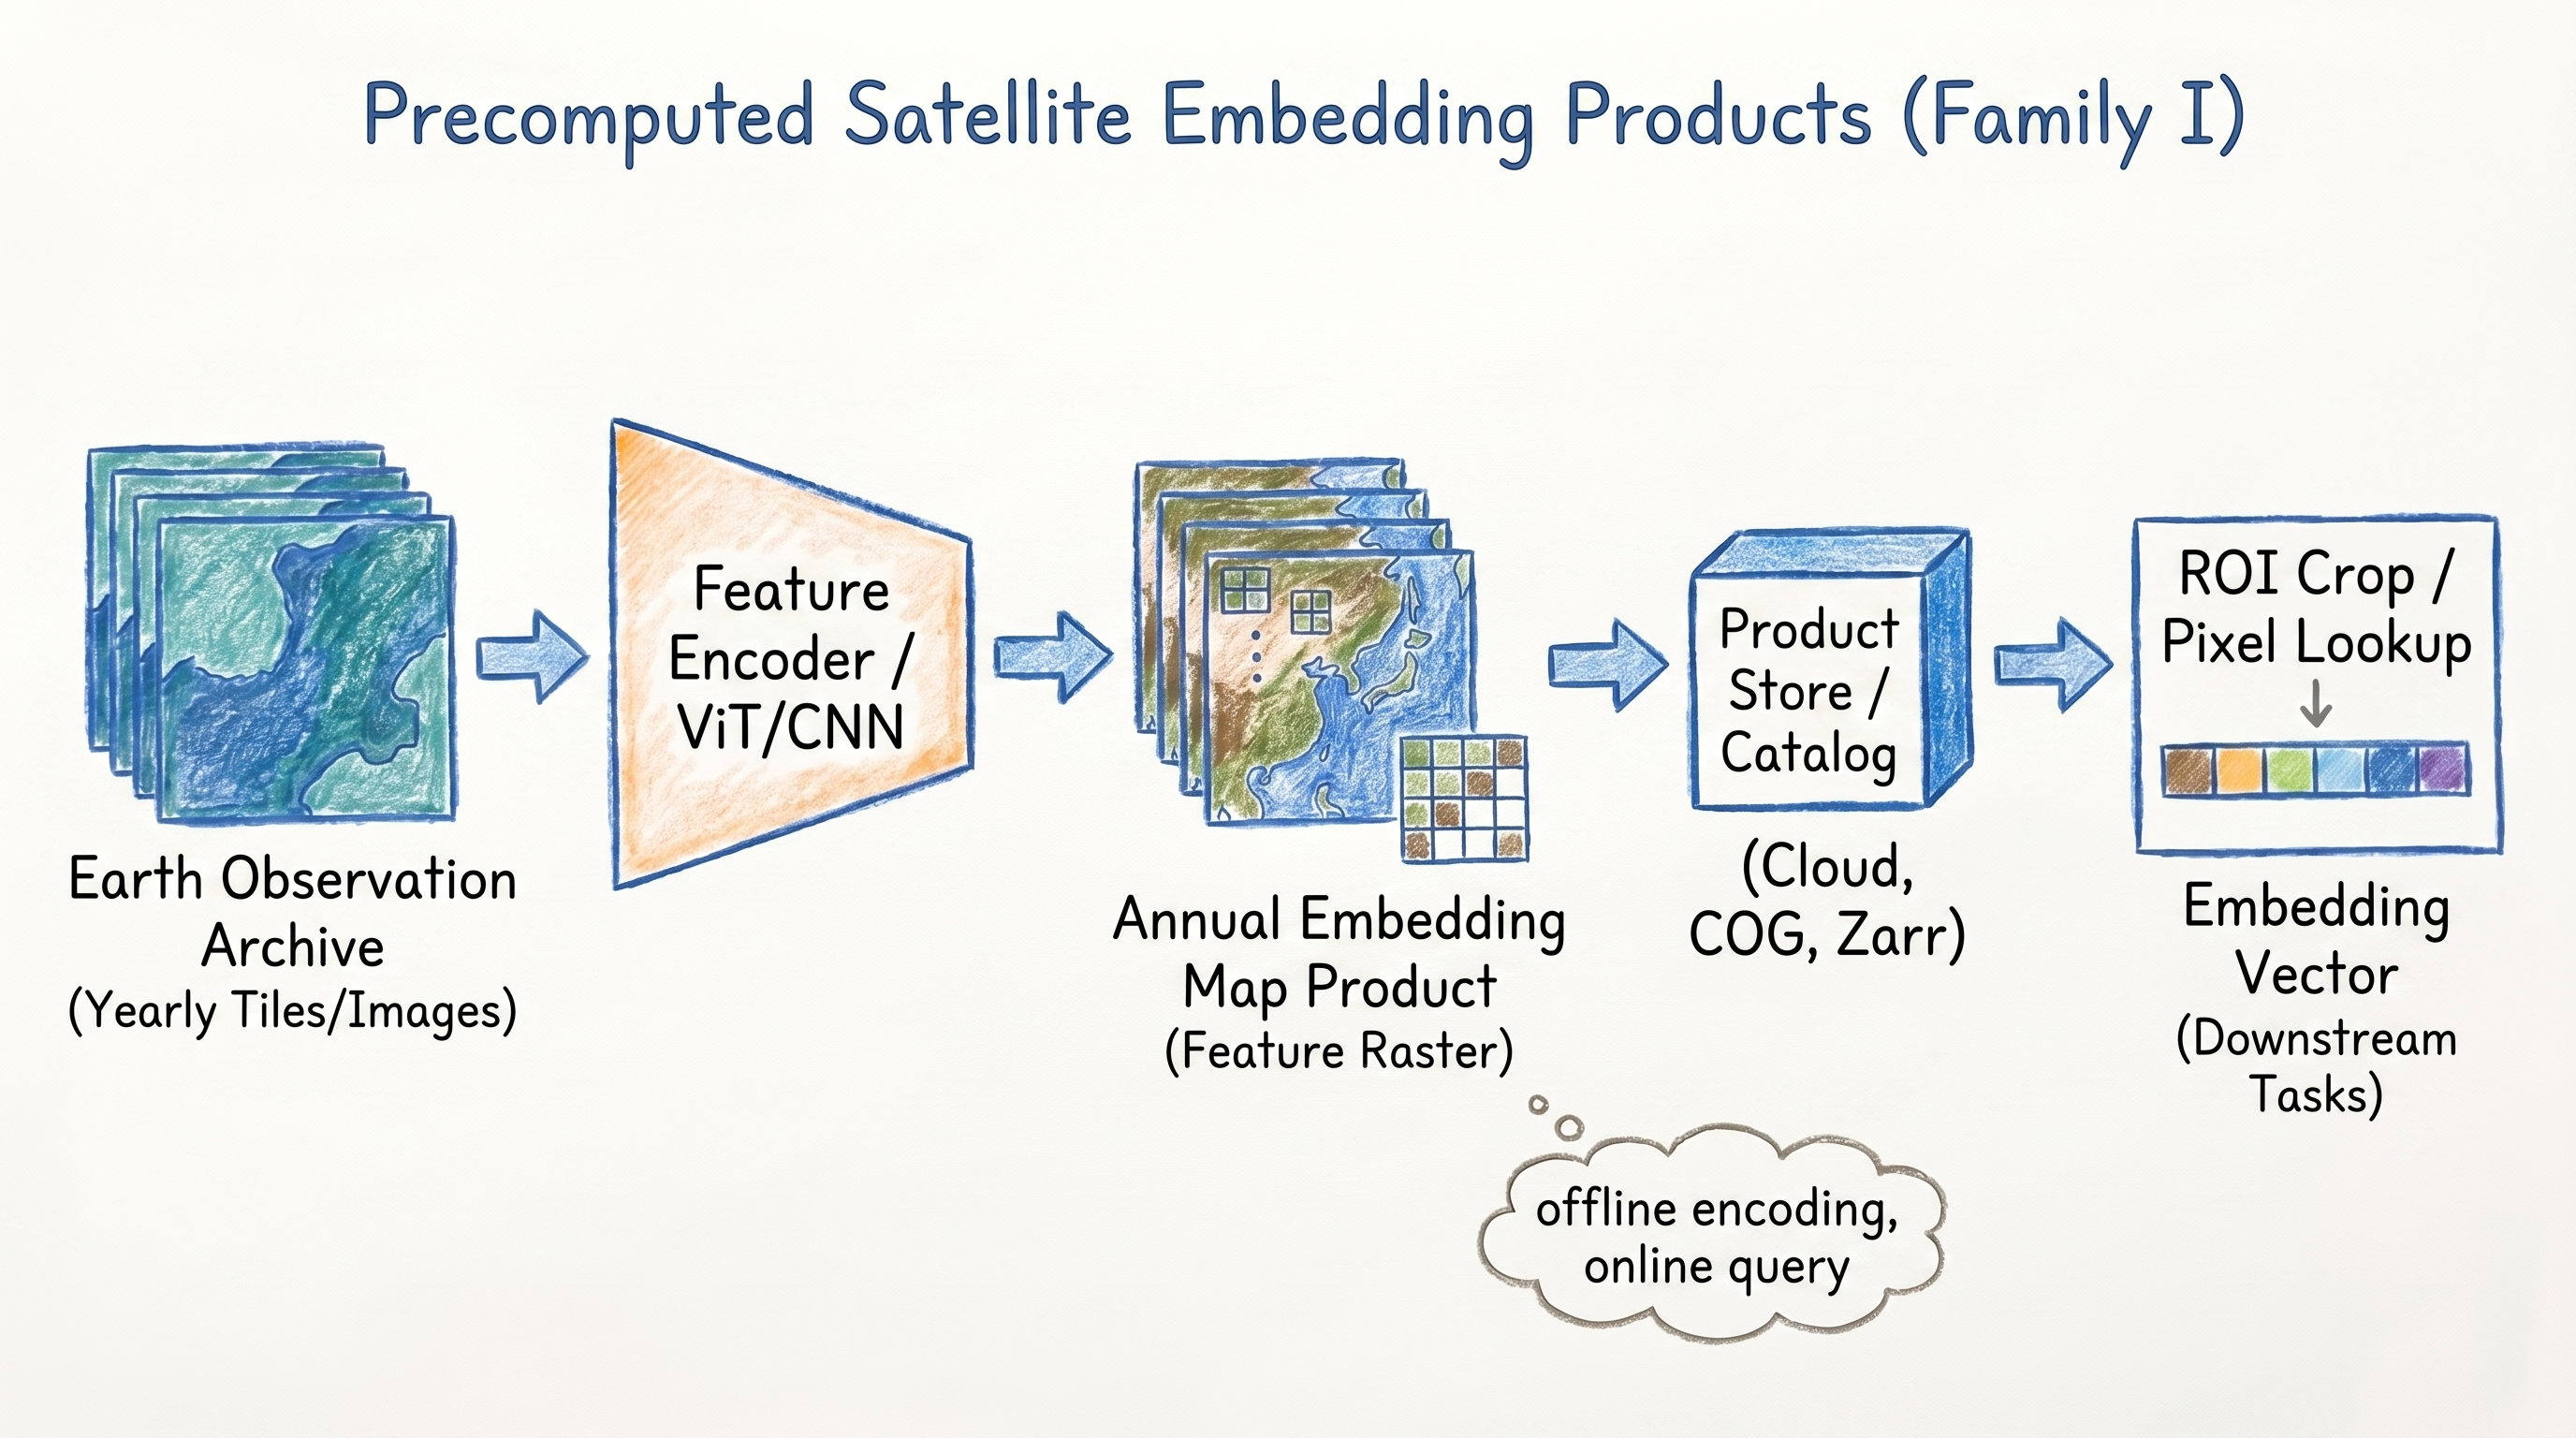
\includegraphics[width=\textwidth]{fig06_family_precomputed_products.png}
  \caption{Unified architecture sketch for precomputed embedding products. The dominant pattern is offline large-scale representation learning followed by annual or static embedding map generation, cataloging, and fast ROI-level feature access.}
  \label{fig:family-precomputed-products}
\end{figure}

\paragraph{Architecture summary.}
The central architectural move is to shift most computation from user-time to production-time. A large Earth observation archive is first condensed into a precomputed feature layer, often annualized or otherwise temporally summarized. Downstream users query that layer by ROI, tile, or pixel rather than rerunning the encoder. This architecture is especially attractive for wide-area monitoring and rapid transfer when access latency matters more than flexible temporal conditioning.

\paragraph{Pseudo-code template.}
\begin{pseudocode}
Input:
  Earth observation archive A
  temporal grouping rule T
  query ROI q

Offline stage:
  train encoder f_theta on large EO archive A
  for each period t in T:
      E_t <- f_theta(A_t)
      store embedding map E_t in product catalog

Online stage:
  crop or sample features z <- E_t[q]
  optionally pool or aggregate z
  train lightweight head g on sampled embeddings
  return prediction or retrieved features
\end{pseudocode}

\subsection{Family II: Masked autoencoder and pure vision encoders}

This group includes models such as SatMAE, SatMAE++, and ScaleMAE \citep{satmae,satmaepp,scalemae}. These methods are usually strongest when the goal is to learn transferable visual structure from optical or multispectral imagery through reconstruction-style pretraining. They are also among the clearest examples of the modern remote sensing foundation model trend, and many later systems can be interpreted as extending this lineage in scale, modality, or temporal handling.

\begin{figure}[t]
  \centering
  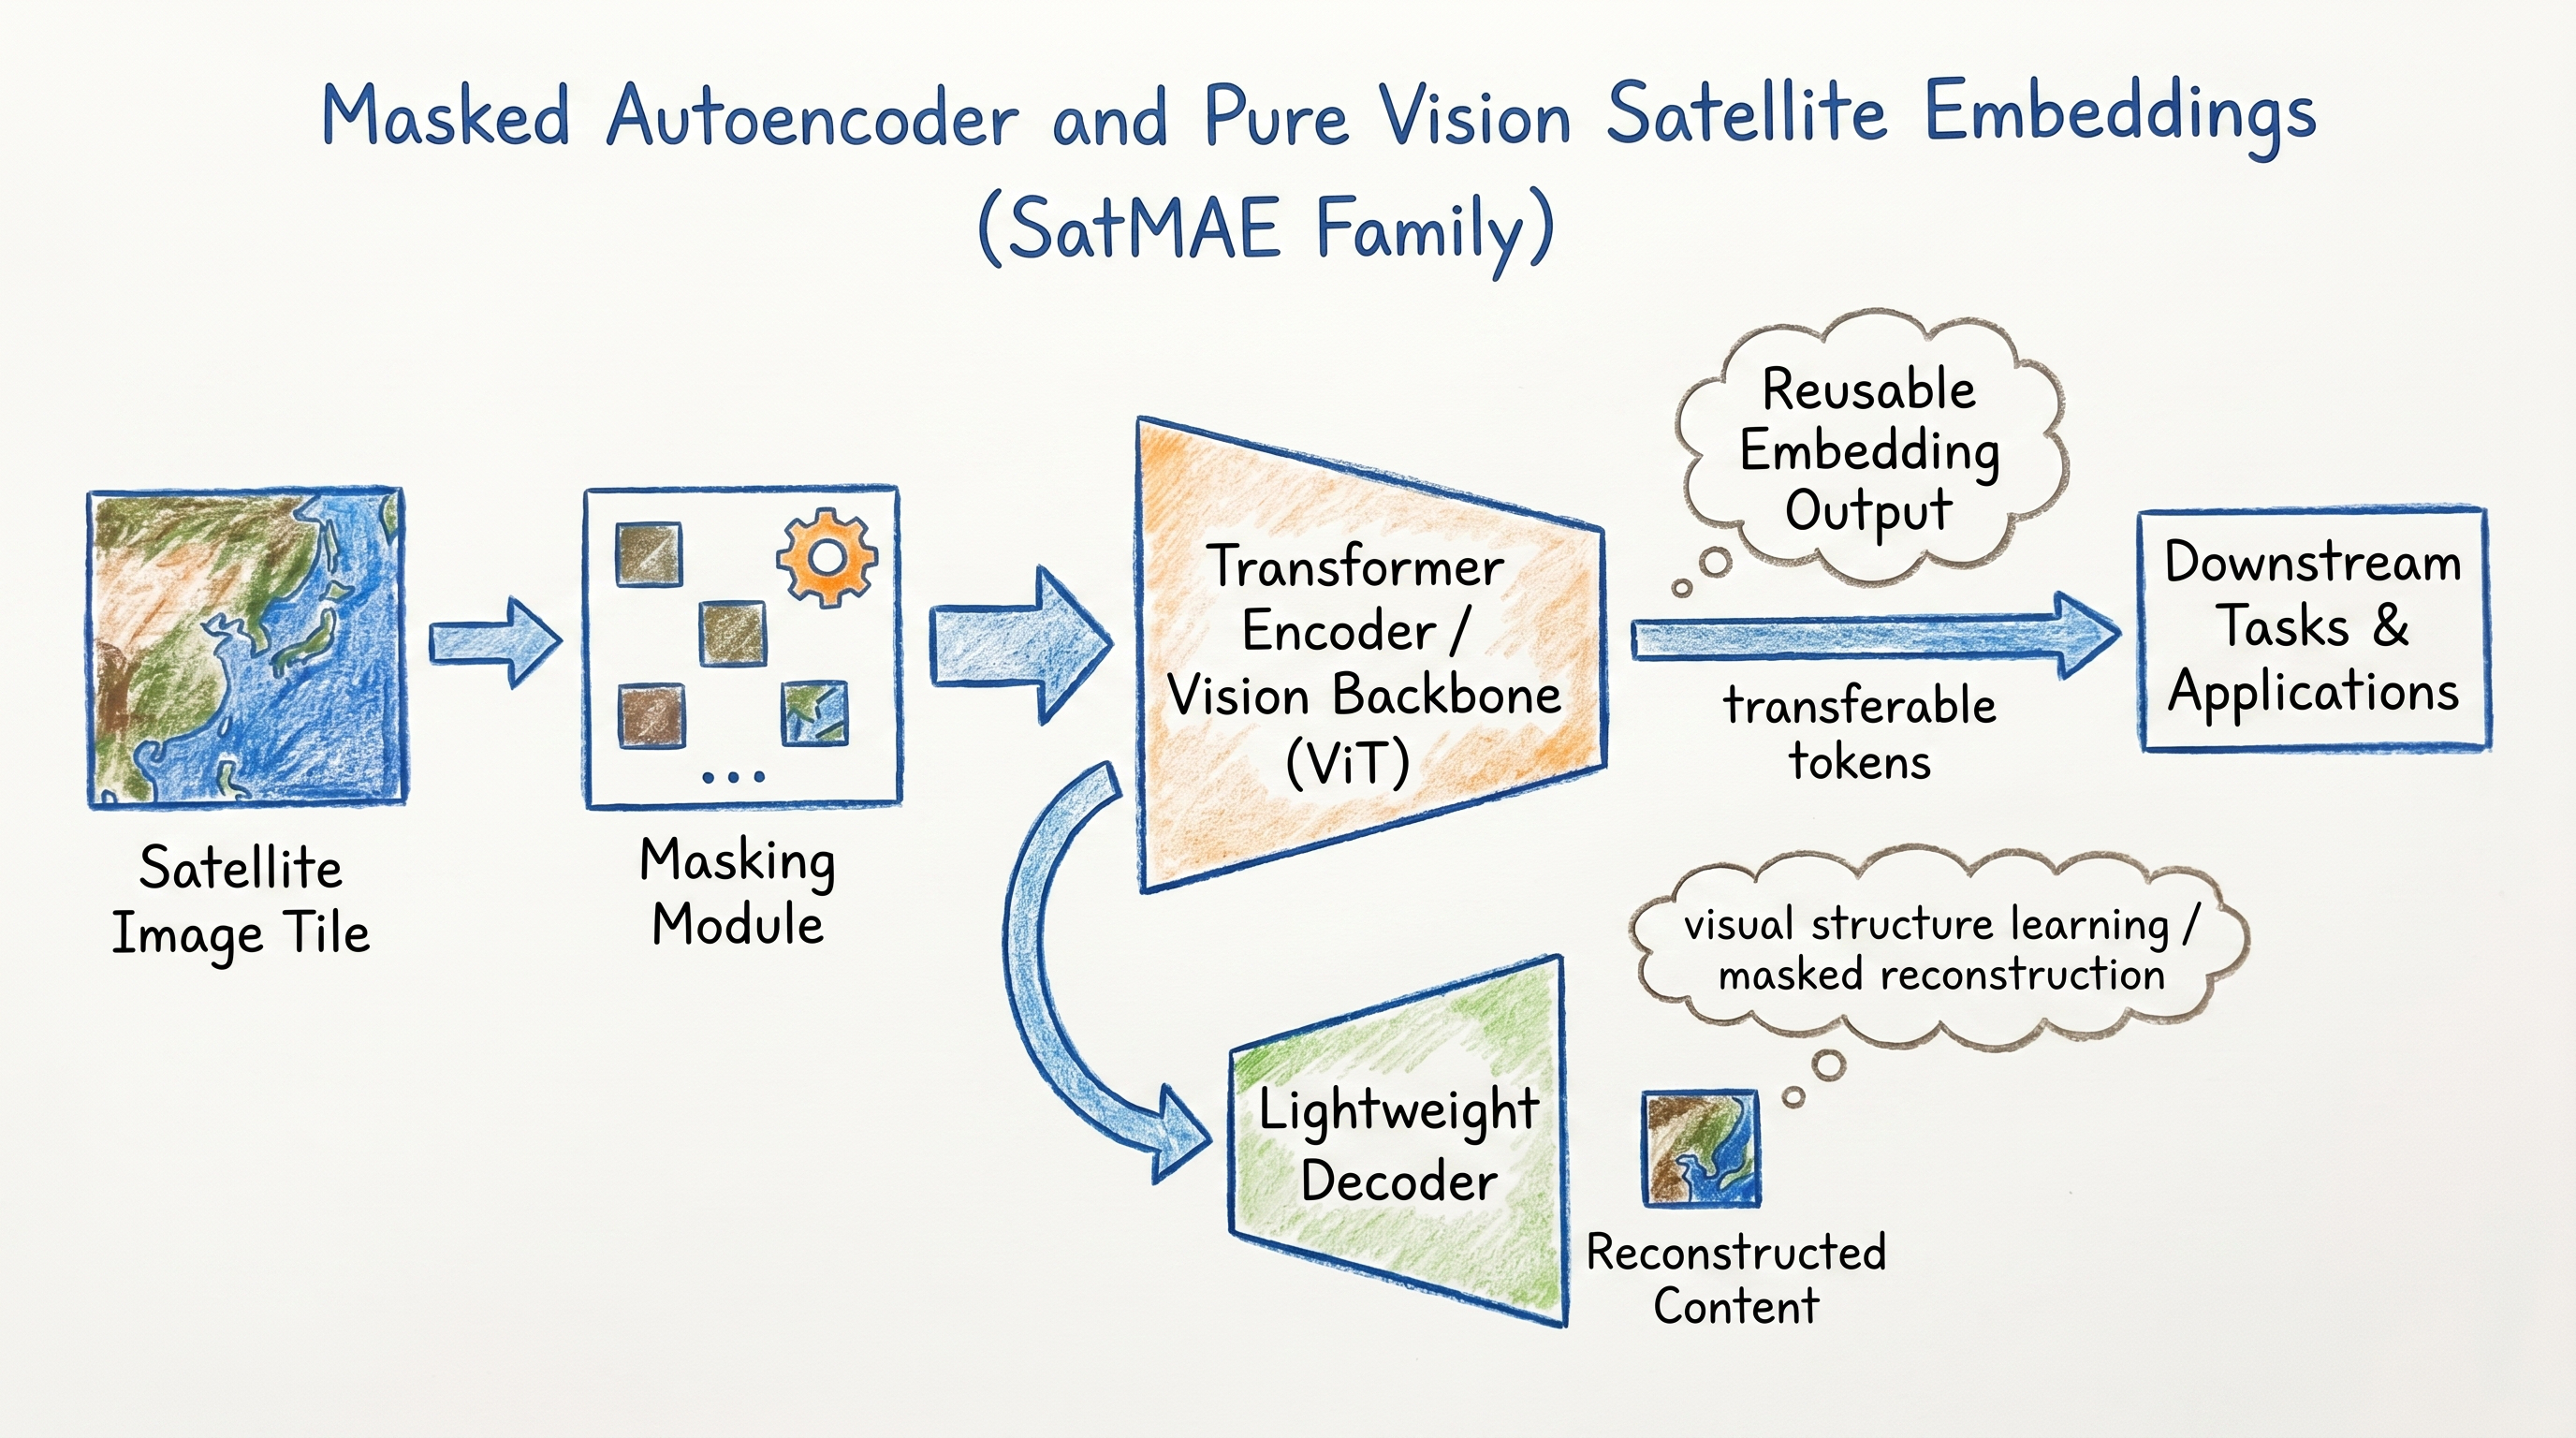
\includegraphics[width=\textwidth]{fig07_family_masked_autoencoder.png}
  \caption{Unified architecture sketch for masked autoencoder and pure vision satellite embedding models. Satellite tiles are partially masked, encoded by a transformer-style vision backbone, and supervised through reconstruction while the latent tokens are reused as transferable embeddings.}
  \label{fig:family-mae}
\end{figure}

\paragraph{Architecture summary.}
The shared logic is to learn a compact latent representation from partial visual evidence. Randomly masked patches, channels, or scale-aware inputs are passed through a vision encoder, while a reconstruction module encourages the latent space to preserve transferable visual structure. These embeddings often work well for classification and segmentation because they retain strong spatial cues without requiring language supervision.

\paragraph{Pseudo-code template.}
\begin{pseudocode}
Input:
  satellite tile x
  masking policy M

visible, hidden <- apply_mask(x, M)
tokens <- patch_embed(visible)
latent <- encoder(tokens)
recon <- decoder(latent, hidden)
loss <- reconstruction_loss(recon, x)
update model parameters

at inference:
  z_pool, z_grid <- read encoder representations
  return transferable embedding features
\end{pseudocode}

\subsection{Family III: Vision-language and cross-modal embeddings}

\begin{figure}[t]
  \centering
  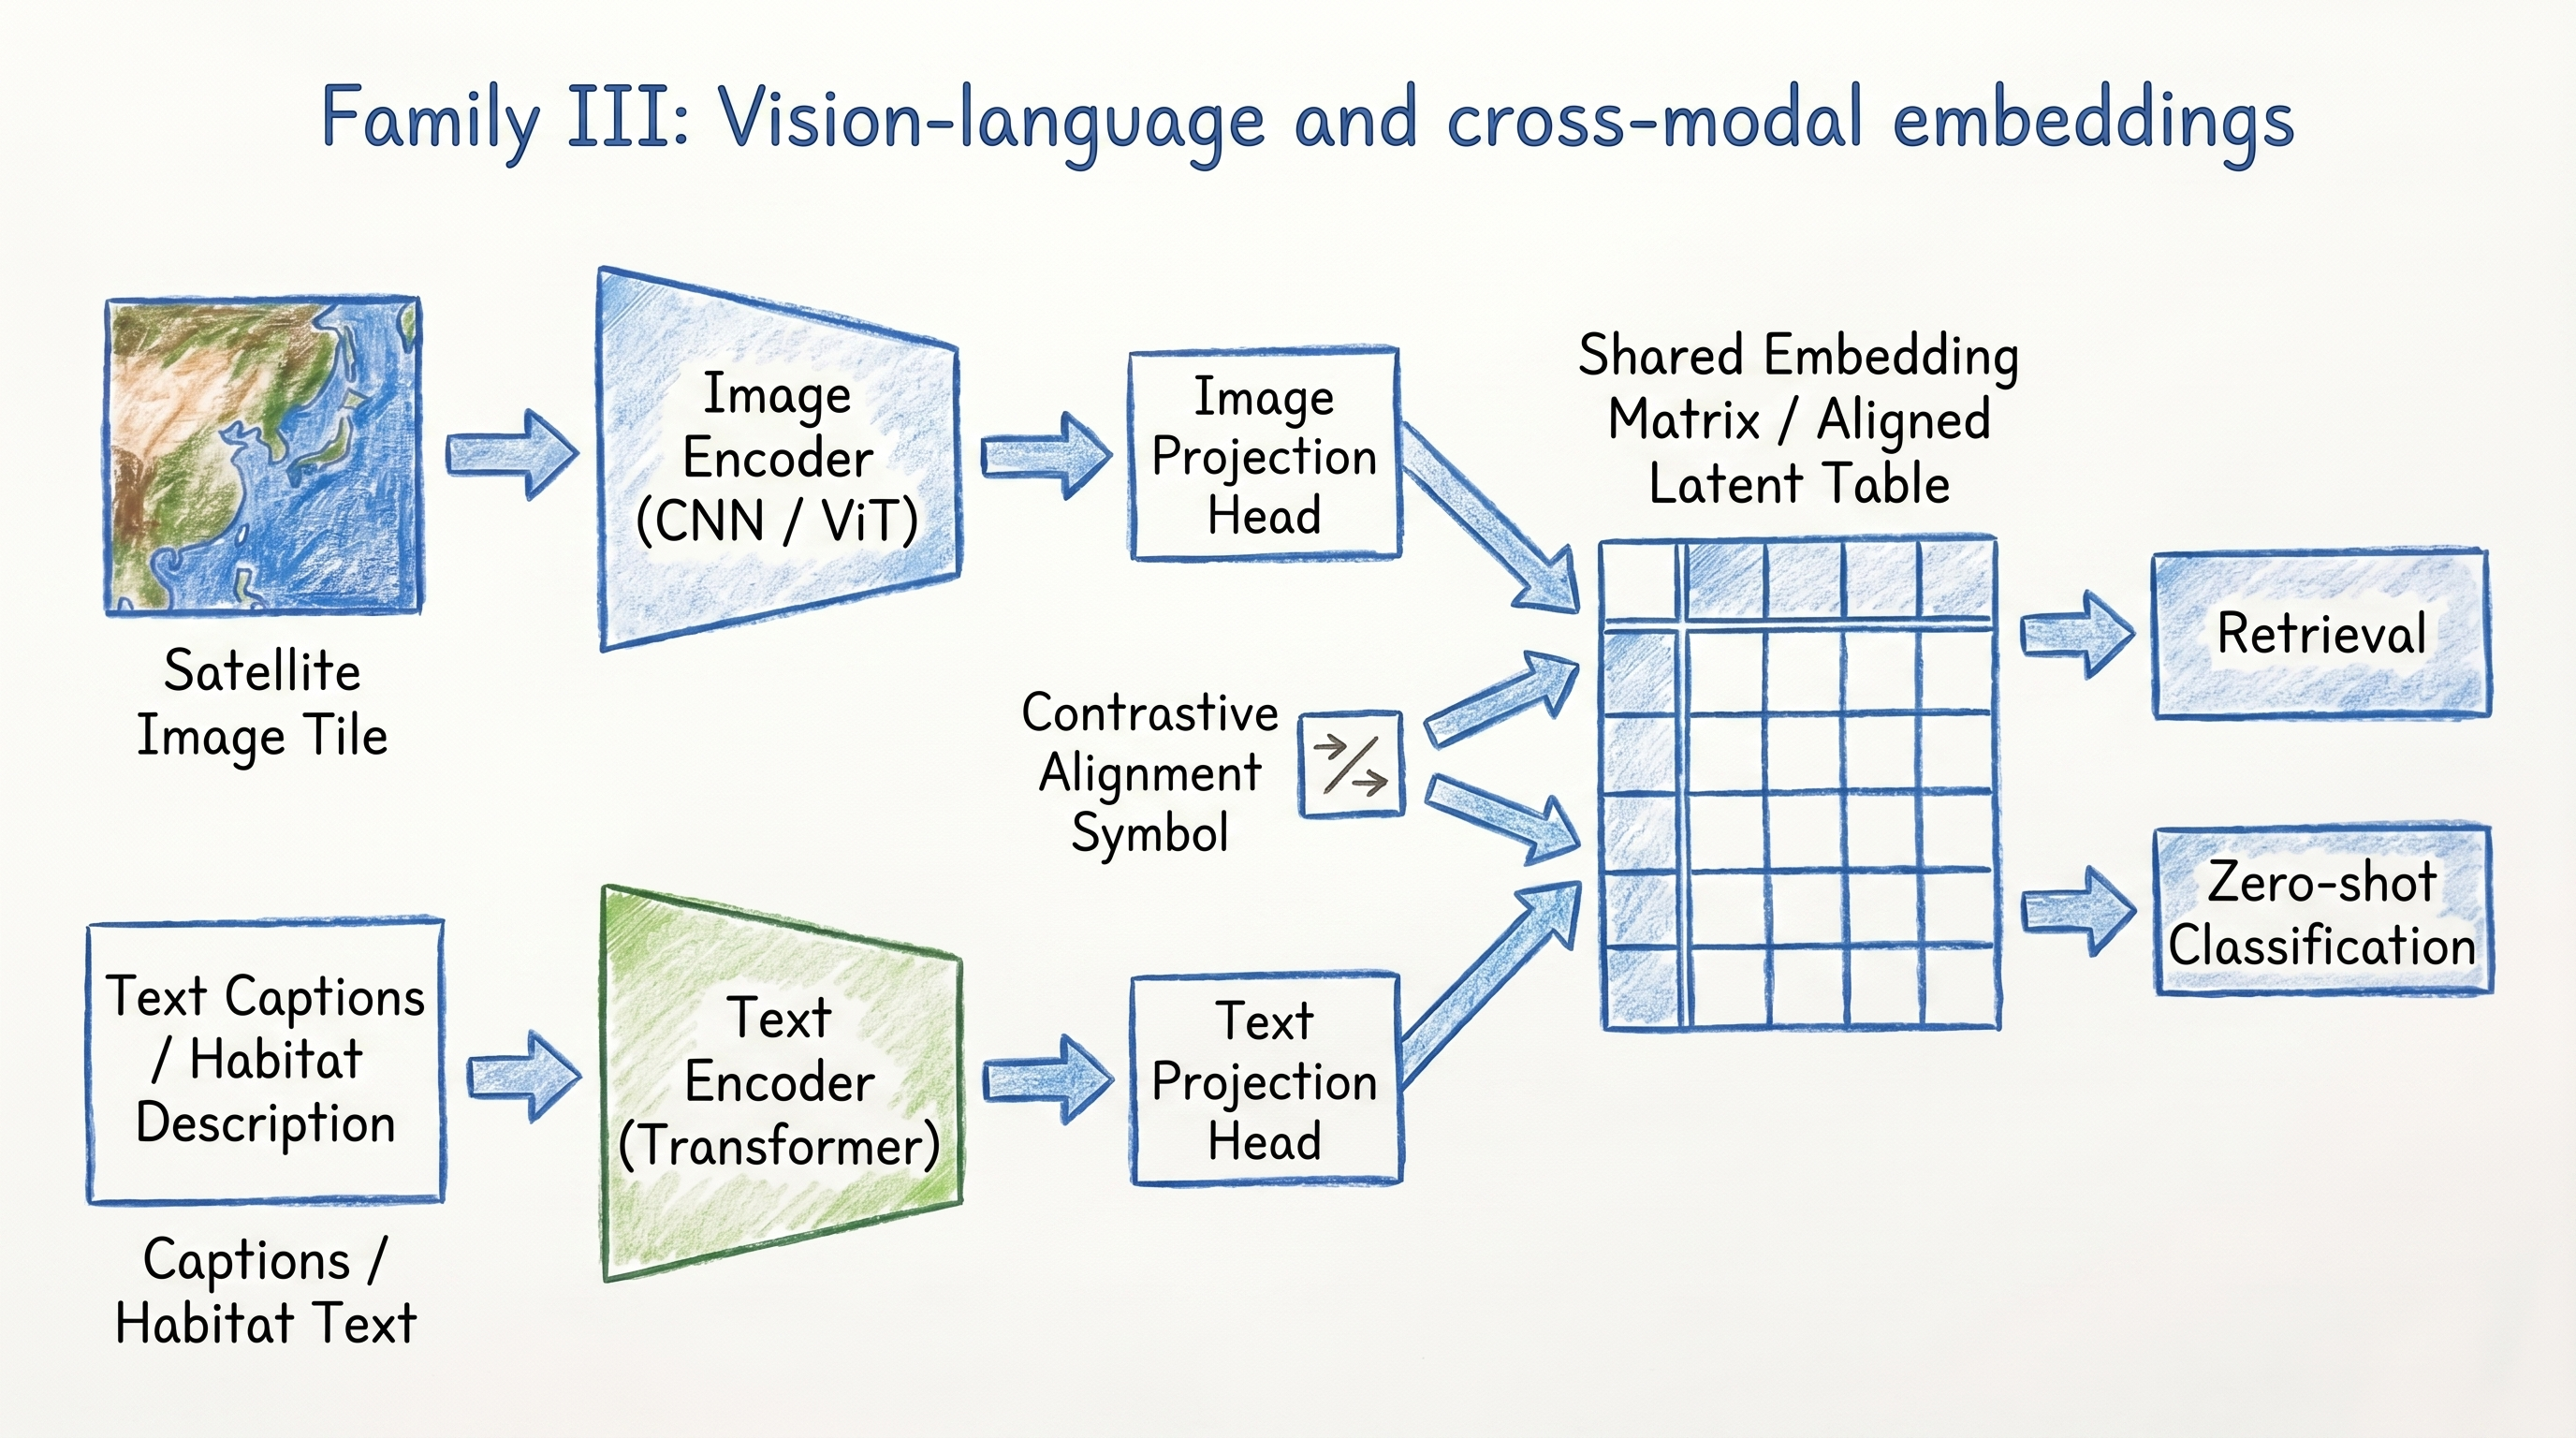
\includegraphics[width=\textwidth]{fig08_family_vision_language.png}
  \caption{Unified architecture sketch for vision-language and cross-modal satellite embeddings. The core pattern is image and text or ecological side-information encoding into a shared latent space trained by contrastive or alignment objectives.}
  \label{fig:family-vision-language}
\end{figure}

RemoteCLIP and WildSAT \citep{remoteclip,wildsat} illustrate the main idea of this family: satellite imagery is no longer embedded only against itself, but aligned with text, captions, habitat descriptions, or ecological side observations. This changes the representation from a purely visual latent space into a semantic one, which is why these models are especially important for retrieval, zero-shot transfer, and open-vocabulary interaction.

\paragraph{Architecture summary.}
Two encoders, one visual and one language or cross-modal, are trained to bring matched image-text or image-side-information pairs closer in a shared embedding space. The representation becomes useful not just for supervised transfer but also for semantic search and weakly supervised reasoning. In practice, this family adds a form of interpretability and open-vocabulary access that reconstruction-only models typically lack.

\paragraph{Pseudo-code template.}
\begin{pseudocode}
Input:
  satellite image x
  text or side-information y

z_img <- image_encoder(x)
z_txt <- text_encoder(y)
loss <- contrastive_alignment(z_img, z_txt)
update both encoders

at inference:
  use z_img for retrieval, zero-shot matching, or downstream probes
  optionally compare z_img against text prompt embeddings
\end{pseudocode}

\subsection{Family IV: Multimodal generalist EO encoders}

AnySat, Galileo, Prithvi, TerraFM, TerraMind, and DOFA represent a broader push toward modality-flexible or sensor-flexible Earth observation representation learning \citep{anysat,galileo,prithvi,terrafm,terramind,dofa}. These models are important because they move the field closer to a genuinely general EO representation space. Their distinguishing features include explicit handling of temporal stacks, wavelength metadata, modality routing, and cross-sensor alignment.

\begin{figure}[t]
  \centering
  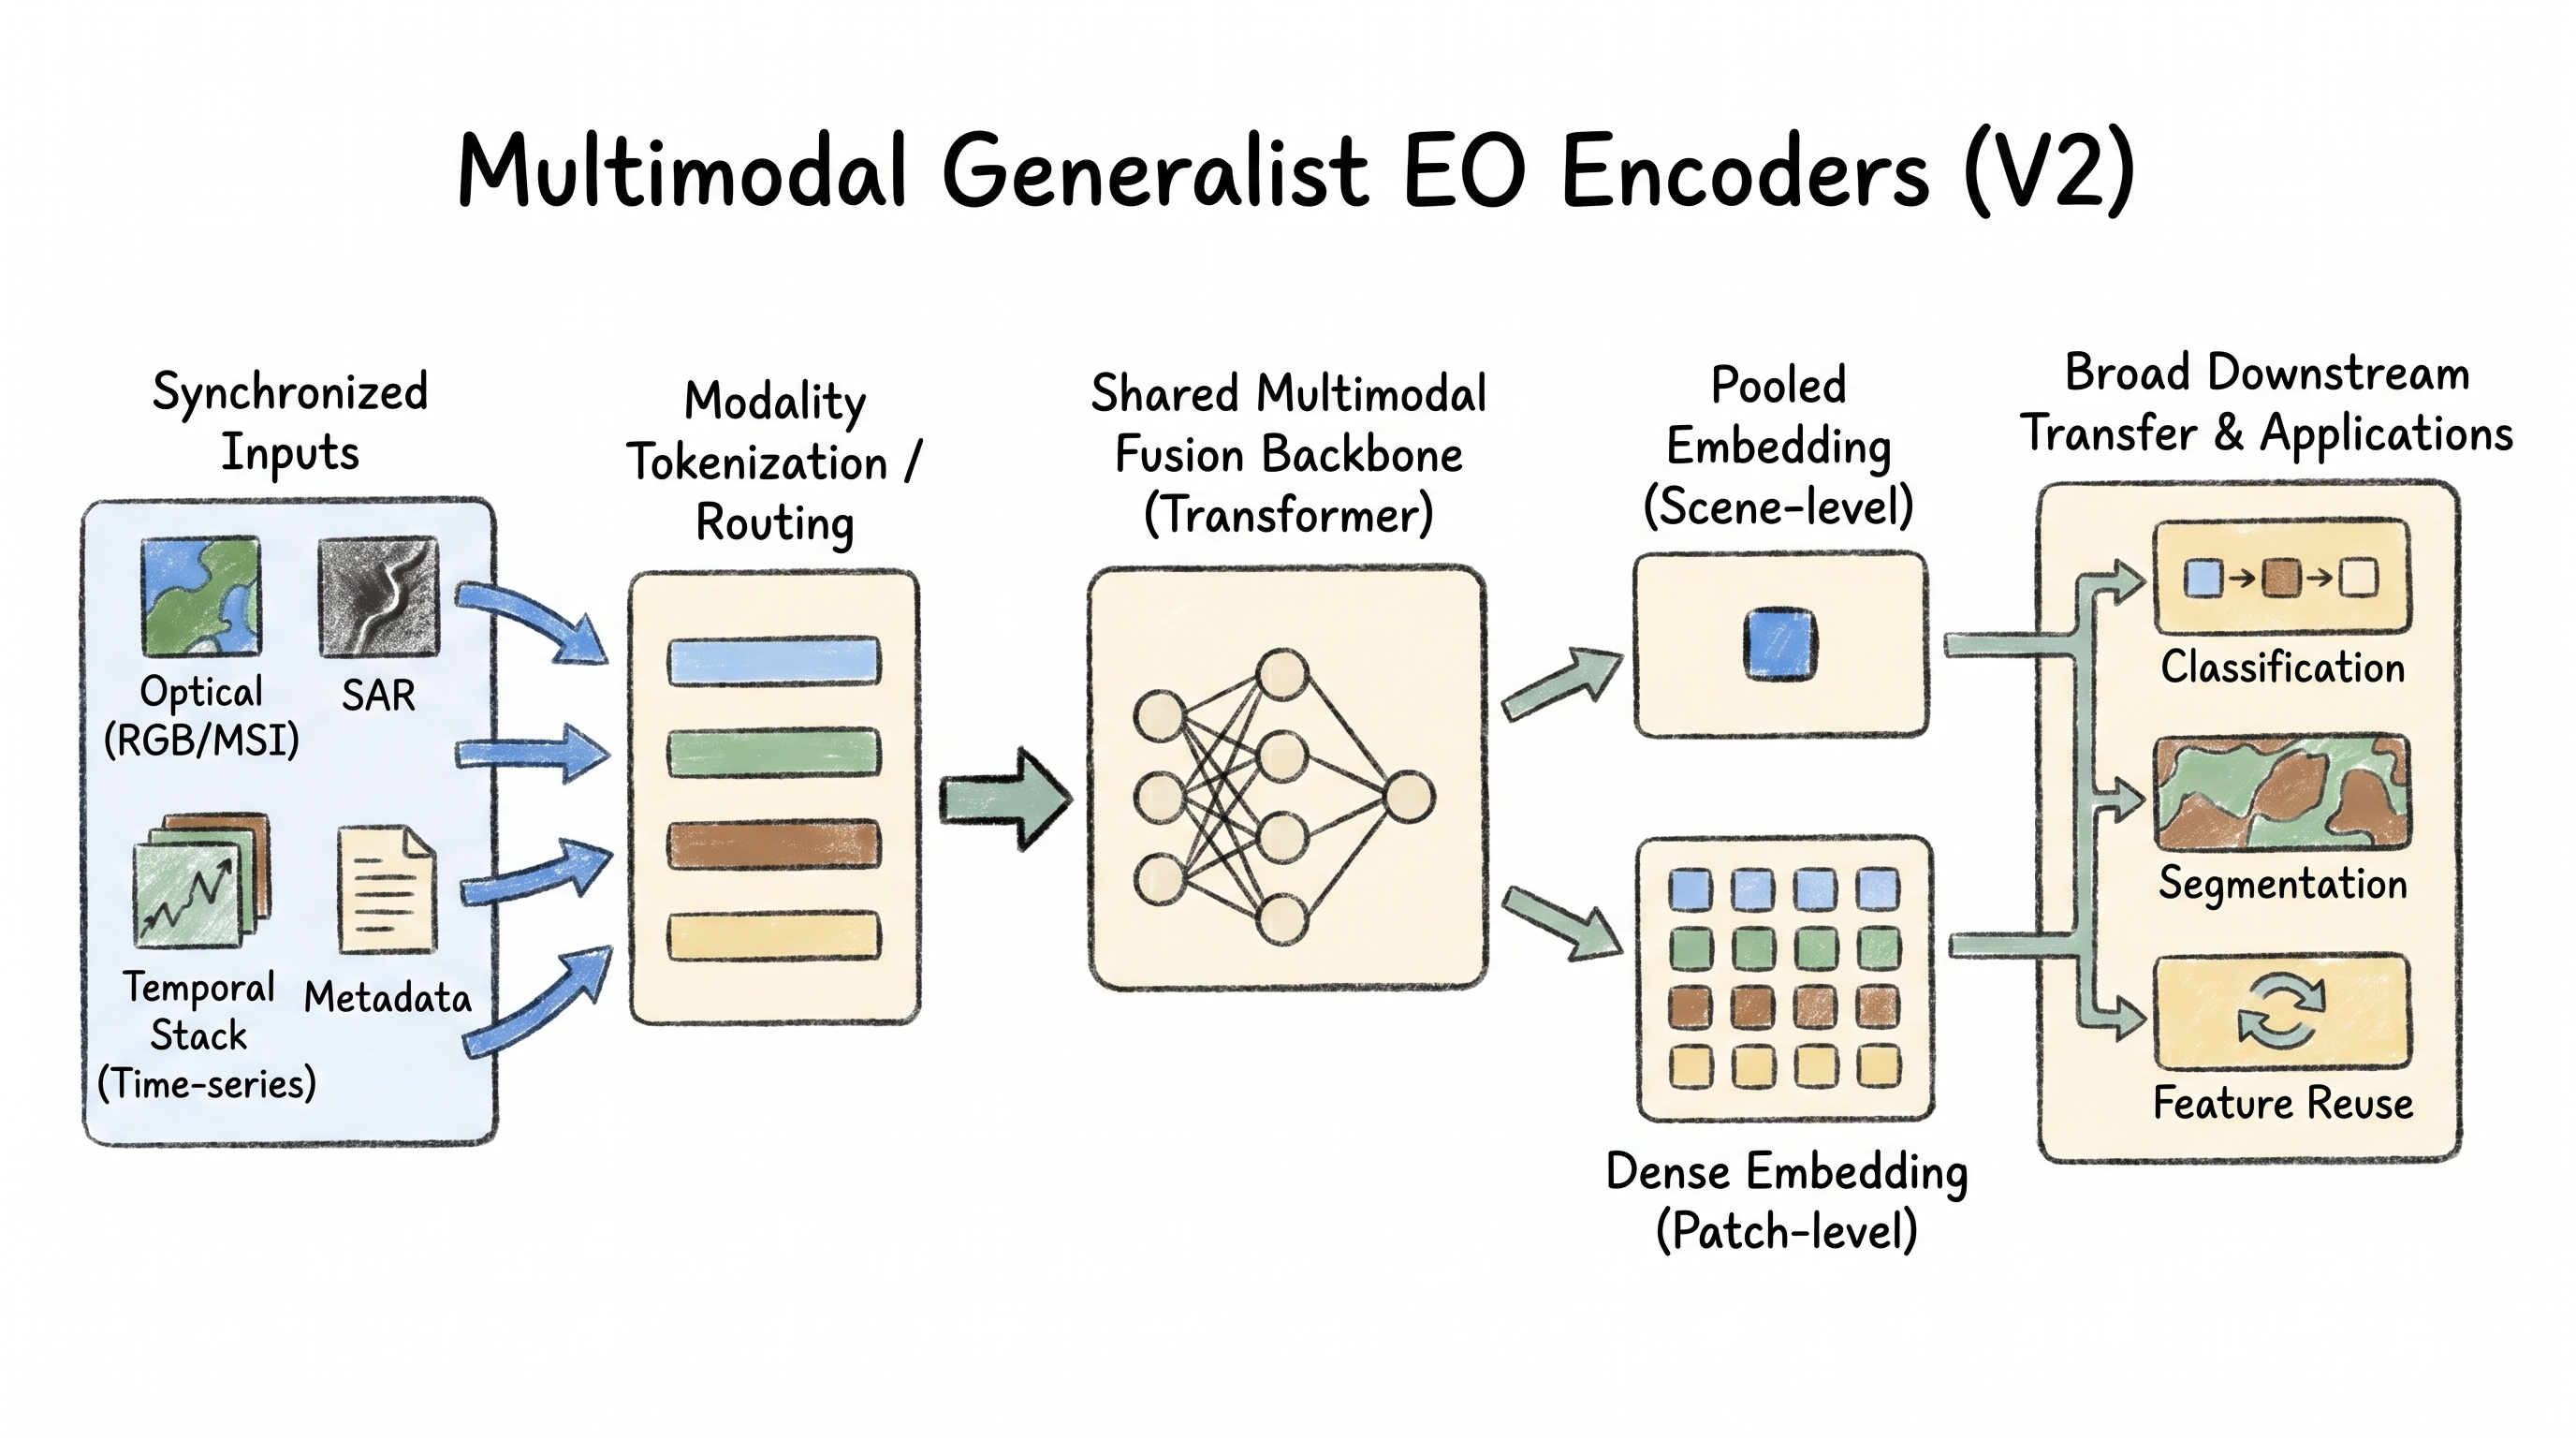
\includegraphics[width=\textwidth]{fig09_family_multimodal_generalist.png}
  \caption{Unified architecture sketch for multimodal generalist EO encoders. Multiple sensor streams are tokenized, routed or aligned, fused by a shared backbone, and exported as pooled or dense representations for broad downstream transfer.}
  \label{fig:family-generalist}
\end{figure}

\paragraph{Architecture summary.}
The defining goal of this family is not simply to process more inputs, but to learn a common representation space across sensors, scales, time, and metadata. Architecturally, that often means modality-specific tokenization combined with a shared transformer or fusion backbone. These models are closest to a true Earth observation foundation layer because they seek one latent space that remains useful under heterogeneous sensing conditions.

\paragraph{Pseudo-code template.}
\begin{pseudocode}
Input:
  modalities {x_1, x_2, ..., x_m}
  temporal or metadata context c

for each modality x_i:
    t_i <- modality_tokenizer_i(x_i, c)

t_shared <- temporal_align_and_route({t_i}, c)
h <- multimodal_backbone(t_shared)
z_pool, z_grid <- readout(h)
optimize self-supervised or multimodal objective

return shared embeddings for cross-sensor downstream transfer
\end{pseudocode}

\subsection{Family V: Domain-specialized embedding models}

Not all useful satellite embeddings aim at maximal generality. AgriFM, FoMo, THOR, and SatVision show that domain-oriented models can remain highly valuable when their sensor assumptions and application context are well matched \citep{agrifm,fomo,thor,satvision}. In a remote sensing review, these models should appear as a major family rather than as outliers, because they often reflect the real structure of EO practice: agriculture, forestry, biodiversity, atmosphere, climate, and societal monitoring all impose different representation demands.

\begin{figure}[t]
  \centering
  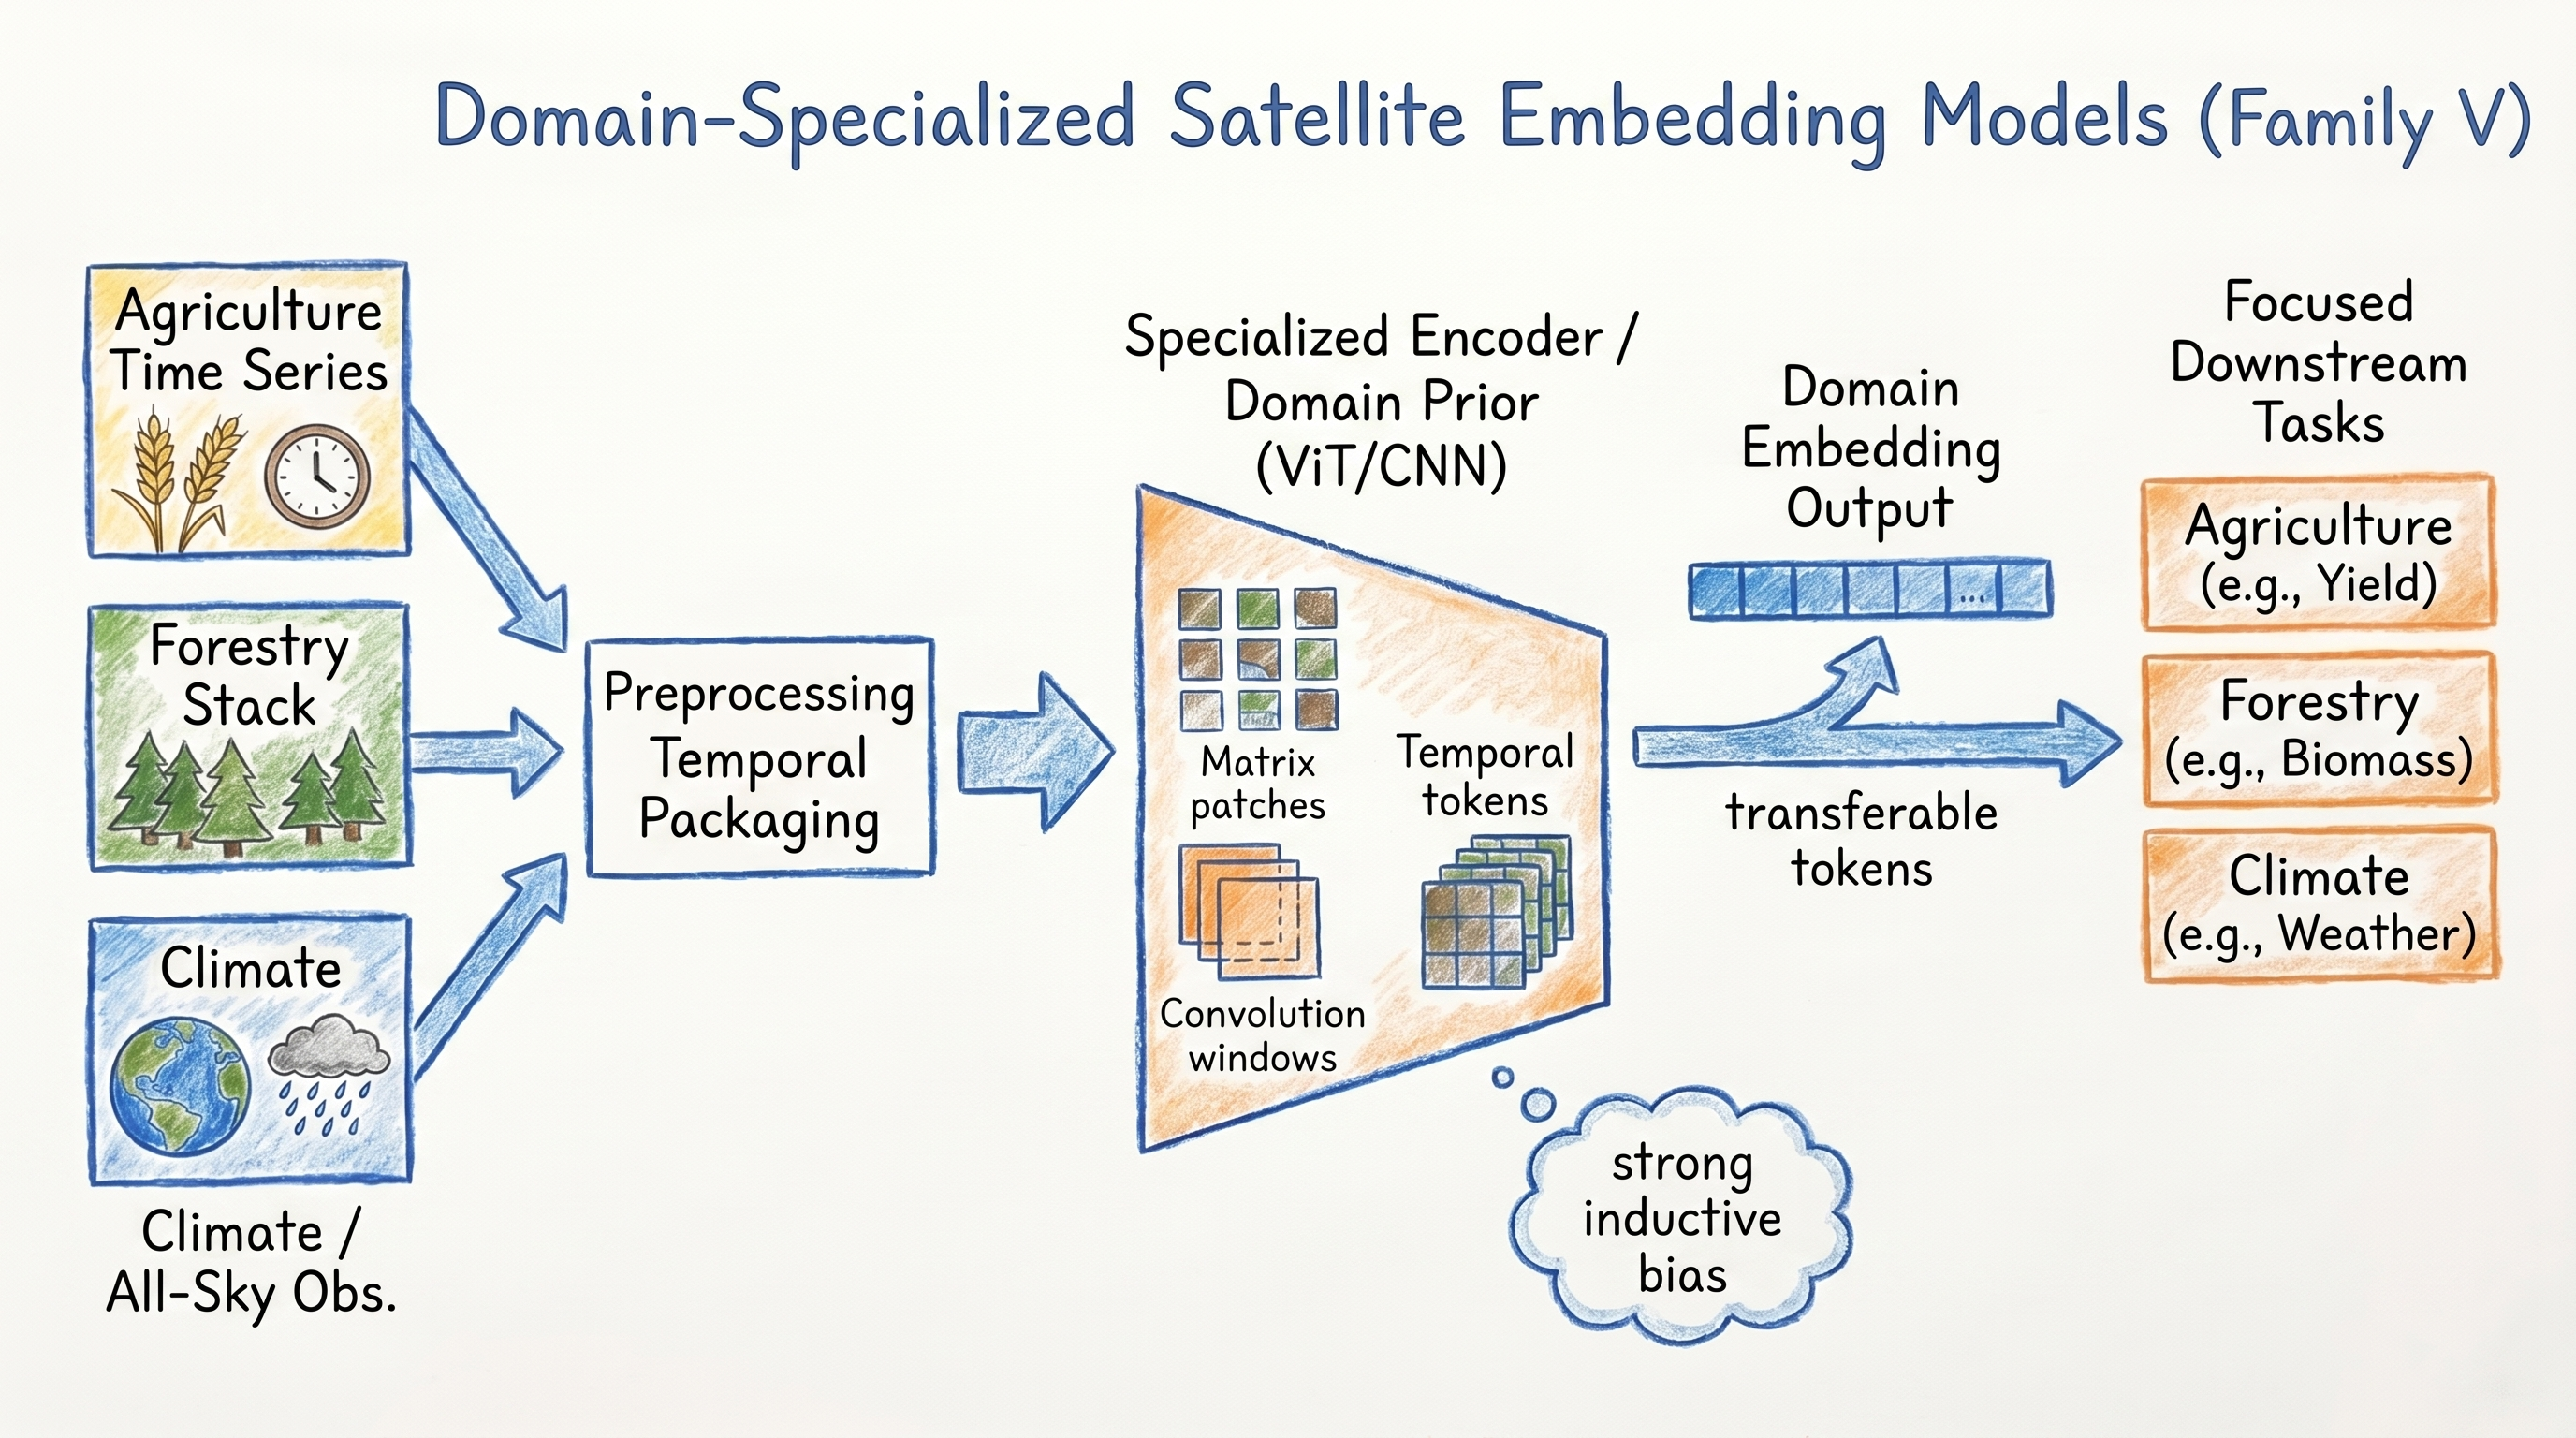
\includegraphics[width=\textwidth]{fig10_family_specialized.png}
  \caption{Unified architecture sketch for domain-specialized satellite embedding models. Domain-specific sensing pipelines and inductive biases are used to produce embeddings that are narrower in scope but often better matched to particular application regimes.}
  \label{fig:family-specialized}
\end{figure}

\paragraph{Architecture summary.}
This family accepts a narrower operating domain in exchange for stronger inductive bias. Agricultural time series, forest monitoring stacks, climate-oriented inputs, or coarse all-sky observations are processed with task-aware temporal packaging, scale handling, or specialized supervision. These models remind us that the best EO embedding is not always the most general one; in many real applications, domain fit matters more than universality.

\paragraph{Pseudo-code template.}
\begin{pseudocode}
Input:
  domain-specific sensor stream x
  domain labels or weak supervision y
  domain prior pi

x_tilde <- domain_preprocess(x, pi)
h <- specialized_encoder(x_tilde, pi)
z <- domain_embedding_head(h)
loss <- domain_objective(z, y, pi)
update model parameters

at deployment:
  reuse z for domain-focused mapping, monitoring, or regression
\end{pseudocode}

\subsection{Cross-family comparison}

After the family-level discussion, the review can return to a unified comparison table. This ordering is closer to the way remote sensing surveys are usually read: first understand the main branches of the field, then inspect the full inventory.

Table~\ref{tab:model-catalog} turns the structured dossier into a paper-ready catalog. Unlike a compact leaderboard, it keeps the deployment type, sensing assumptions, temporal semantics, and pretraining regime visible, because these details strongly determine whether a model is suitable for retrieval, dense prediction, or operational mapping. Appendix Table~\ref{tab:model-appendix-catalog} extends this inventory with authorship, task hints, runtime, GPU memory, and implementation-facing metadata.

\begin{landscape}
\scriptsize
\setlength{\LTleft}{0pt}
\setlength{\LTright}{0pt}
\setlength{\tabcolsep}{3pt}
\renewcommand{\arraystretch}{1.15}
\begin{longtable}{p{1.45cm}p{0.75cm}p{1.2cm}p{0.95cm}p{2.25cm}p{2.05cm}p{2.75cm}p{2.35cm}p{2.25cm}p{1.55cm}p{3.0cm}}
\caption{Comprehensive model summary for the \modelcount{} canonical satellite embedding models currently exposed in \texttt{rs-embed}. The table emphasizes deployment-relevant details rather than only benchmark scores.}\label{tab:model-catalog}\\
\toprule
Model & Year & Venue & Type & Family & Backbone & Sensors / data & Resolution & Temporal semantics & Emb. / output & Pretraining signal \\
\midrule
\endfirsthead
\caption[]{Comprehensive model summary for the canonical \texttt{rs-embed} model set (continued).}\\
\toprule
Model & Year & Venue & Type & Family & Backbone & Sensors / data & Resolution & Temporal semantics & Emb. / output & Pretraining signal \\
\midrule
\endhead
\bottomrule
\endfoot
tessera & 2026 & CVPR & precomputed & Precomputed temporal embedding field & field model over surface spectra embeddings & surface spectra product & 10 m precomputed embedding tiles & annual lookup over product years & 128; pooled, grid & embedding field regression / product training \\
gse & 2025 & arXiv & precomputed & Precomputed annual embedding product & embedding field model & Google Satellite Embedding annual product & 10 m annual embedding product & strict yearly product & 64; pooled, grid & global embedding field learning from sparse labels \\
copernicus & 2025 & ICCV & precomputed & Precomputed foundation map & Copernicus foundation model product & Copernicus product stack & 0.25\textdegree{} precomputed grid & static in current adapter (2021 only) & 768; pooled, grid & foundation model pretraining followed by product distillation \\
remoteclip & 2024 & IEEE TGRS & on-the-fly & Vision-language satellite embedding & CLIP / ViT-B-32 & Sentinel-2 RGB, remote sensing captions, UAV imagery in pretraining & 10 m; Sentinel-2 RGB & single composited observation window at inference & 768; pooled, grid & contrastive image-text alignment (InfoNCE) \\
satmae & 2022 & NeurIPS & on-the-fly & Masked autoencoder for temporal or multispectral EO & ViT-MAE & Sentinel-2 RGB or multispectral/time-series variants in original paper & 10 m; Sentinel-2 RGB & explicit temporal embeddings in the original paper; rs-embed adapter currently uses RGB composite path & 1024; pooled, grid & masked autoencoding with temporal/spectral positional encoding \\
satmaepp & 2024 & CVPR & on-the-fly & Improved masked autoencoder for EO & ViT-L / SatMAE++ & Sentinel-2 RGB in adapter, multispectral Sentinel-2 in paper & 10 m; Sentinel-2 RGB & single composited observation window in adapter & 1024; pooled, grid & revised MAE pretraining for multispectral satellite imagery \\
satmaepp\_s2\_10b & 2024 & CVPR & on-the-fly & Grouped-channel multispectral masked autoencoder & ViT-L / grouped-channel SatMAE++ & Sentinel-2 SR 10-band & 10 m; Sentinel-2 SR 10-band input & single composited observation window in adapter & 1024; pooled, grid & grouped-channel masked autoencoding \\
scalemae & 2023 & ICCV & on-the-fly & Scale-aware masked autoencoder & ViT-L / MAE & Sentinel-2 RGB in adapter, multiscale EO imagery in paper & 10 m; Sentinel-2 RGB, plus explicit semantic scale input & single composited observation window & 1024; pooled, grid & masked autoencoding with explicit resolution conditioning \\
anysat & 2025 & CVPR & on-the-fly & Generalist multi-resolution multimodal EO encoder & versatile JEPA-style EO encoder & Sentinel-2, Sentinel-1, aerial/VHR and other modalities in original paper & 10 m Sentinel-2 time-series input; default per-frame resize 24 px & multi-frame optical sequence with date tokens & 768; pooled, grid & self-supervised representation learning across many configurations \\
galileo & 2025 & ICML & on-the-fly & Global-local multimodal time-series encoder & transformer with global/local branches & Sentinel-2 time series, multiple remote sensing modalities in original work & 10 m Sentinel-2 time-series input; default frame size 64 px, patch size 8 & explicit month tokens and frame masks & 128; pooled, grid & self-supervised multimodal representation learning \\
wildsat & 2025 & ICCV & on-the-fly & Remote sensing representation learning from weak labels & ViT-B-16 & Sentinel-2 RGB, wildlife observations as supervision & 10 m; Sentinel-2 RGB & single composited optical patch & 256; pooled, grid & supervised / weakly supervised representation learning from wildlife observations \\
prithvi & 2023 & arXiv & on-the-fly & Generalist geospatial foundation model & ViT / masked autoencoder lineage & HLS / Sentinel-Landsat style 6-band optical imagery & 30 m in current adapter; Sentinel-2 6-band input & explicit temporal coordinates in adapter and paper family & 768; pooled, grid & self-supervised geospatial pretraining \\
terrafm & 2026 & ICLR & on-the-fly & Unified multisensor foundation model & multisensor transformer & Sentinel-2, Sentinel-1 & 10 m for both S2 and S1 paths; image resized to 224 px & single observation window in current adapter; paper focuses on multisensor unification & 768; pooled, grid & scalable unified multisensor pretraining \\
terramind & 2025 & ICCV & on-the-fly & Generative multimodal EO foundation model & large-scale generative multimodal transformer & Sentinel-2 in adapter, wider multimodal EO stack in paper & 10 m; Sentinel-2 SR 12-band input; image resized to 224 px & single composited optical path in adapter & 384; pooled, grid & large-scale generative multimodal learning \\
dofa & 2024 & arXiv & on-the-fly & Wavelength-aware multimodal foundation model & transformer with neural plasticity / dynamic wavelength handling & multispectral and hyperspectral style inputs, Sentinel-2 in adapter & 10 m for S2 path; fixed resize to 224 px & single observation window in adapter & 768; pooled, grid & self-supervised multimodal EO foundation modeling \\
fomo & 2025 & AAAI & on-the-fly & Forest-oriented multimodal and multiscale foundation model & multimodal transformer / representation learner & Sentinel-2 SR in adapter, multiple scales and tasks in original work & 10 m; Sentinel-2 SR 12-band input; default image size 64 px & single optical composite in adapter & 768; pooled, grid & multi-task forest monitoring pretraining \\
thor & 2026 & arXiv & on-the-fly & Versatile EO foundation model for climate and society & versatile transformer & Sentinel-2 SR 10-band & 10 m; Sentinel-2 SR 10-band input; default image size 288 px & single optical composite in adapter & 768; pooled, grid & foundation pretraining for climate and society applications \\
agrifm & 2026 & Remote Sensing of Environment & on-the-fly & Agriculture-specific multi-source temporal foundation model & Video Swin Transformer & Sentinel-2 in adapter, Sentinel-2, Landsat-8/9, MODIS in original paper & 10 m Sentinel-2 time-series input; default image size 224 px with fixed T-frame packaging & fixed-length multi-frame temporal stack & 1024; pooled, grid & supervised land-cover fraction pretraining with EMA teacher \\
satvision & 2024 & arXiv & on-the-fly & Coarse-resolution all-sky foundation model & SwinV2-style encoder & MODIS 14-band TOA & 1000 m; 14-channel TOA input & single coarse-resolution observation window in adapter & 4096; pooled, grid & foundation pretraining on all-sky MODIS TOA data \\
\end{longtable}
\normalsize
\end{landscape}


Three contrasts recur across families. First, precomputed layers prioritize access and coverage, while on-the-fly encoders prioritize flexibility. Second, multimodal and time-aware systems attempt to absorb sensor heterogeneity at training time, whereas narrower families often compensate with stronger specialization and simpler deployment. Third, vision-language models add open-vocabulary semantics that are mostly absent from pure masked reconstruction pipelines. These contrasts matter more for a review paper than a single benchmark leaderboard, because they explain why different families remain competitive under different downstream conditions.

\begin{figure}[t]
  \centering
  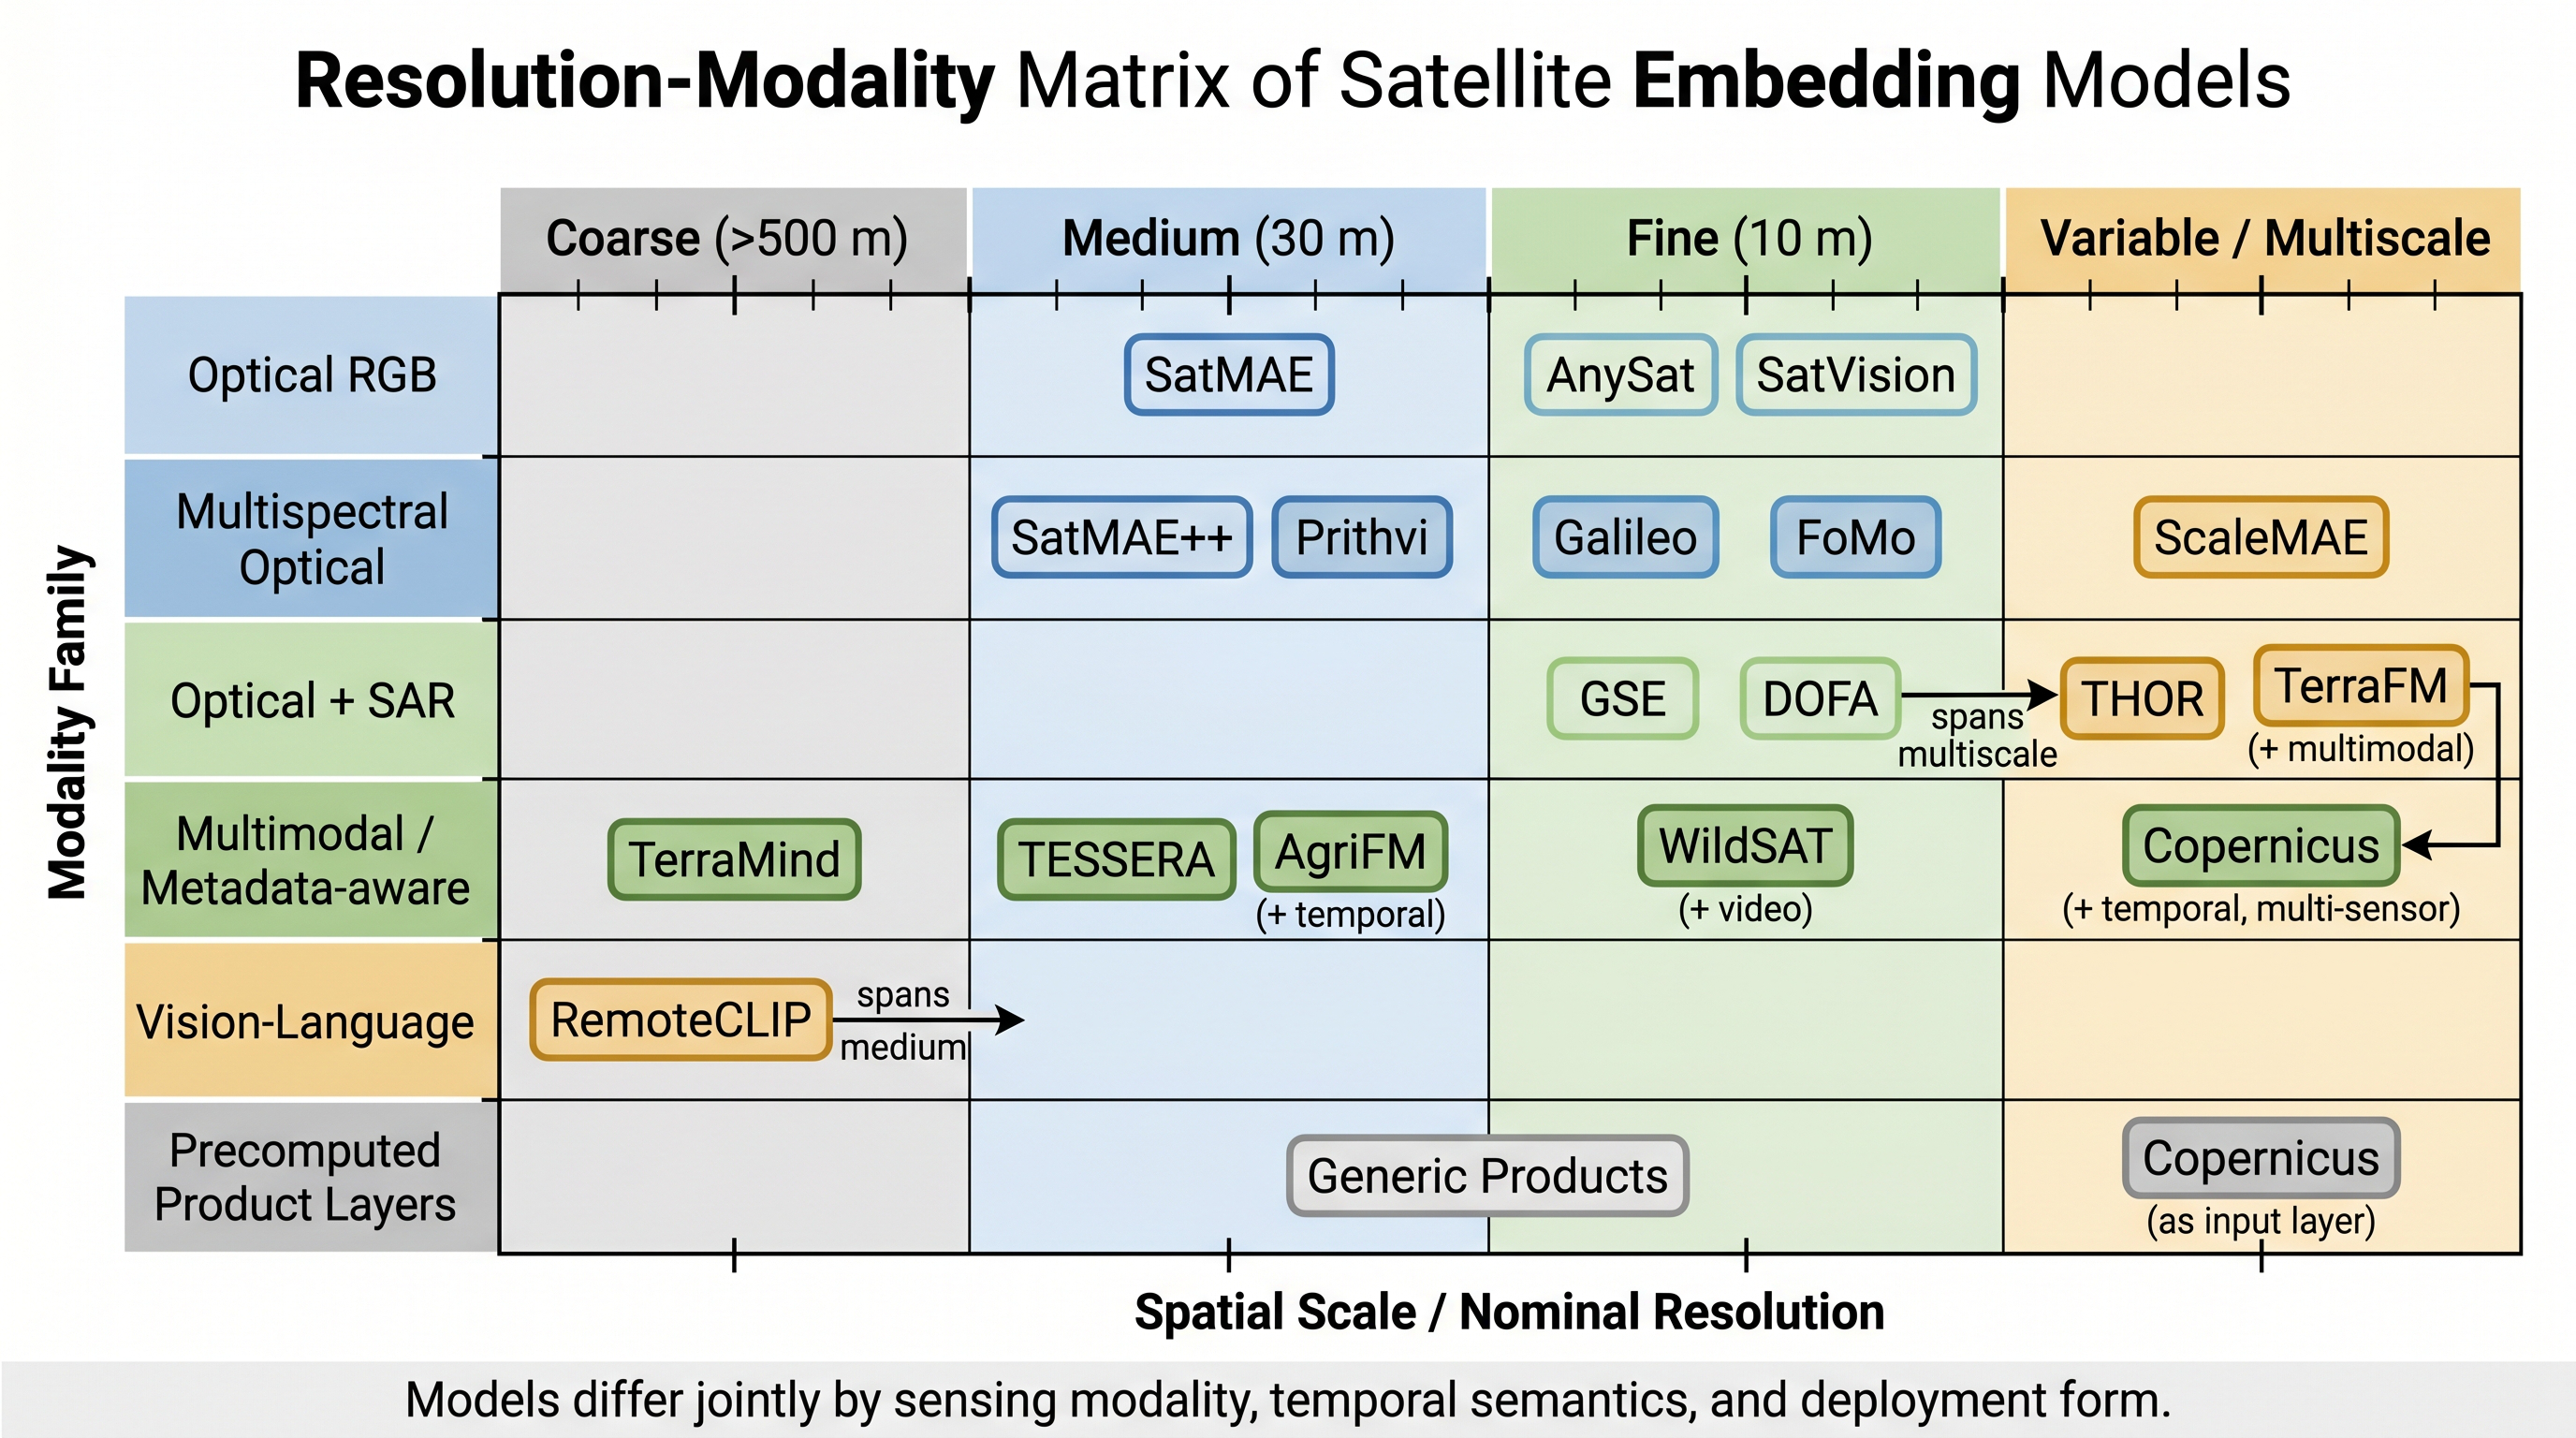
\includegraphics[width=\textwidth]{fig05_resolution_modality_matrix.png}
  \caption{Resolution-modality matrix for current satellite embedding models. The same model family can occupy very different parts of the sensing space, from coarse-resolution all-sky imagery to high-resolution optical-SAR or multimodal temporal embeddings.}
  \label{fig:resolution-modality-matrix}
\end{figure}

Figure~\ref{fig:resolution-modality-matrix} closes this section by summarizing the sensing space covered by current models. In a remote sensing context, this figure is often more informative than a single ranking table because it makes sensor assumptions and scale mismatch immediately visible.
